\documentclass[conference]{IEEEtran}
\IEEEoverridecommandlockouts
% Based on the IEEE conference template (Overleaf):
% https://www.overleaf.com/latex/templates/ieee-conference-template/grfzhhncsfqn
\usepackage{cite}
\usepackage{amsmath,amssymb,amsfonts}
\usepackage{graphicx}
\usepackage{textcomp}
\usepackage{xcolor}
\usepackage{booktabs}
\usepackage{placeins}
\usepackage{tikz}
\usetikzlibrary{arrows.meta,positioning,shapes.geometric,fit,calc}
\usepackage[hidelinks]{hyperref}
\def\BibTeX{{\rm B\kern-.05em{\sc i\kern-.025em b}\kern-.08em
    T\kern-.1667em\lower.7ex\hbox{E}\kern-.125emX}}

\graphicspath{{figs/}}

\tikzset{
  blk/.style={draw, rounded corners=2pt, align=center, font=\footnotesize, minimum height=7mm, inner sep=3pt},
  proc/.style={draw, align=center, font=\scriptsize, minimum width=34mm, minimum height=5.5mm, inner sep=2pt},
  dec/.style={draw, diamond, aspect=2.6, align=center, font=\scriptsize, inner sep=0.5pt},
  term/.style={draw, rounded corners=7pt, align=center, font=\scriptsize, minimum width=22mm, minimum height=5.5mm},
  arr/.style={-{Stealth[length=2mm]}, thick},
}

\begin{document}

\title{Vibration-Based Structural Damage Detection Using an ARM Cortex-M3 Microcontroller}

\makeatletter
\newcommand{\linebreakand}{%
  \end{@IEEEauthorhalign}
  \hfill\mbox{}\par
  \mbox{}\hfill\begin{@IEEEauthorhalign}
}
\makeatother

\author{
\IEEEauthorblockN{Sagnik Basu}
\IEEEauthorblockA{Reg. No. 240953528\\
Roll No. 42}
\and
\IEEEauthorblockN{Pranav Gaddam}
\IEEEauthorblockA{Reg. No. 240953548\\
Roll No. 43}
\and
\IEEEauthorblockN{Shobit Hegde}
\IEEEauthorblockA{Reg. No. 240953556\\
Roll No. 44}
\linebreakand
\IEEEauthorblockA{School of Computer Engineering\\
Section CCE A\\
Manipal Institute of Technology, Manipal, India}
}

\maketitle

\begin{abstract}
Structural health monitoring (SHM) reveals damage before it leads to failure, but most vibration-based systems rely on costly acquisition hardware and a computer for analysis. The natural frequency, the most widely used damage indicator, is also blind to some faults and shifts under harmless changes such as added mass. Recent TinyML studies mostly target powerful processors, so a complete, verified pipeline on a basic microcontroller is missing. This paper presents a damage detection system that runs entirely on an LPC1768 ARM Cortex-M3. An MPU6050 MEMS accelerometer records the free vibration of a steel cantilever at 100 Hz. The firmware computes a windowed 1024-point FFT with parabolic peak interpolation and a log-envelope damping estimate, then runs a decision tree, k-nearest neighbours, a 5-8-4 neural network, a health score and a change detector, all trained offline and exported as C code. On 89 laboratory recordings covering a healthy state, added mass, loose joints and support loosening, the neural network reached 93.8\% cross-validated accuracy against 84.2\% for a frequency-only rule. The health score erred by 5.6 points on average, and board and PC outputs matched on every recording. Damping, not frequency, exposed support loosening. Explainable SHM therefore fits in 20 KB of flash on an entry-level microcontroller.
\end{abstract}

\begin{IEEEkeywords}
ARM Cortex-M3, edge machine learning, MEMS accelerometer, structural health monitoring, TinyML, vibration-based damage detection
\end{IEEEkeywords}

%=====================================================================
\section{Introduction}
%=====================================================================
Civil and mechanical structures lose stiffness over time through cracks, corrosion and loosened connections. Structural health monitoring (SHM) aims to detect such damage automatically, ideally before it becomes visible, by answering four questions in order: is there damage, where is it, what type is it, and how severe is it~\cite{gharehbaghi2022}. Vibration-based methods are attractive because any change in stiffness, mass or boundary condition alters the dynamic response of the structure, which can be measured with a single accelerometer~\cite{hou2021,avci2021}.

The classical indicator is the first natural frequency. It is cheap to compute and global, but it has two known weaknesses. First, many faults barely change it, and second, harmless changes such as added mass or temperature shift it as much as real damage~\cite{hou2021}. Machine learning (ML) addresses both by combining several features and learning the pattern of each condition from data~\cite{avci2021,flah2021,bao2021}. However, most ML-based SHM pipelines are trained and run on a PC or in the cloud, which needs a continuous data link and dedicated acquisition hardware~\cite{malekloo2022,zonzini2020}.

Tiny machine learning (TinyML) moves inference onto the microcontroller next to the sensor~\cite{ray2022,capogrosso2024}. This reduces data traffic, power and cost, but most published SHM work at the edge uses multi-core or DSP-capable chips and neural networks that are hard to explain. This work asks a simpler question: can a complete, explainable damage detection pipeline, from raw acceleration to a named fault and a health score, run on an entry-level ARM Cortex-M3 with no floating-point unit and a 32 KB code limit, and can its results be verified on real hardware?

The contributions of this paper are:
\begin{enumerate}
\item An assemble-only cantilever test bench made from two steel rulers, binder clips and a screw clamp, on which three fault types are introduced repeatably and without tools.
\item Fixed-point-friendly firmware for the LPC1768 that samples an MPU6050 at 100 Hz and extracts five features, including interpolated frequency and log-envelope damping, with a self-written radix-2 FFT.
\item Six lightweight models (decision tree, kNN, 5-8-4 neural network, kNN health regression, z-score change detector and novelty detector) trained on a laptop and exported automatically as C code.
\item An experimental study on 89 recordings showing that the ML outperforms a frequency-only rule, that damping is the only usable indicator of support loosening, and that board and PC outputs are identical.
\end{enumerate}

%=====================================================================
\section{Literature Review}
%=====================================================================
\subsection{Vibration-based damage identification}
Hou and Xia~\cite{hou2021} reviewed a decade of vibration-based damage identification for civil structures. They group methods by the feature used, such as natural frequencies, mode shapes, damping and frequency response functions, and note that frequency is the easiest to measure but the least informative about the type and location of damage. Gharehbaghi \emph{et al.}~\cite{gharehbaghi2022} formalise the SHM levels and compare model-based and data-driven approaches. Both reviews stress that environmental and operational changes can mask or mimic damage, which motivates the added-mass test used in this work.

\subsection{Machine learning for SHM}
Avci \emph{et al.}~\cite{avci2021} trace the move from hand-set thresholds to ML and deep learning, showing that a feature-extraction stage followed by a classifier is the dominant structure. Flah \emph{et al.}~\cite{flah2021} systematically review supervised and unsupervised algorithms in civil SHM and identify small labelled datasets as the main obstacle. Bao and Li~\cite{bao2021} describe ML as a new paradigm for SHM covering damage identification, data anomaly detection and condition assessment. Malekloo \emph{et al.}~\cite{malekloo2022} survey ML together with emerging sensing technology, including low-cost MEMS sensors and IoT nodes. Closest to this work, de Sousa \emph{et al.}~\cite{desousa2023} compared kNN, support vector machines, decision trees, random forests and naive Bayes for classifying damage in cantilever beams. Using natural-frequency indices alone their accuracy ranged from about 59\% to 94\%, while richer response features reached about 95\% on experimental data, showing that frequency alone is not enough.

\subsection{Loosening as a fault}
Loosened supports and bolted joints are among the most common faults in real structures. Huang \emph{et al.}~\cite{huang2022} review loosening detection for threaded fasteners and report that vibration-based methods detect it through changes in stiffness and in energy dissipation at the contact interface, that is, through both frequency and damping. This motivates the damping feature used here.

\subsection{Frequency estimation}
With a finite record, the FFT resolves frequency only to $\Delta f = F_s/N$. Belega and Petri~\cite{belega2021} show that fitting a parabola through the three largest DTFT samples around a peak estimates the frequency far more accurately than the peak bin alone, at almost no extra cost. This technique is used on the board.

\subsection{SHM at the edge and TinyML}
Zonzini \emph{et al.}~\cite{zonzini2020} propose a sensor-to-cloud SHM architecture in which MEMS sensor nodes pre-process data before sending it. Ray~\cite{ray2022} and Capogrosso \emph{et al.}~\cite{capogrosso2024} review TinyML frameworks, model compression and deployment on microcontrollers. In SHM specifically, Burrello \emph{et al.}~\cite{burrello2022} train tiny autoencoders to detect anomalies near the sensor, Moallemi \emph{et al.}~\cite{moallemi2023} accelerate output-only system identification on a parallel RISC-V microcontroller, and Capello \emph{et al.}~\cite{capello2025} use neural architecture search to fit SHM models on resource-constrained devices.

\subsection{Research gap}
Table~\ref{tab:lit} summarises the closest works. Existing edge SHM studies use capable processors and anomaly-only or black-box models, while the beam classification studies run on a PC. None of them combines fault-type classification, a severity score and a change detector on a basic Cortex-M3, verified against real data with bit-level agreement between the PC and the board.

\begin{table}[t]
\caption{Comparison with closely related work}
\label{tab:lit}
\centering
\footnotesize
\setlength{\tabcolsep}{3pt}
\begin{tabular}{@{}lllll@{}}
\toprule
Work & Platform & Output & Features & Data \\
\midrule
\cite{desousa2023} & PC & fault class & freq., FRF & sim.\,+\,exp. \\
\cite{burrello2022} & MCU (multi-core) & anomaly & raw signal & real \\
\cite{moallemi2023} & RISC-V MCU & modal param. & AR/ARMA & real \\
\cite{capello2025} & MCU & anomaly & learned & real \\
This work & Cortex-M3 & class, health, & freq., damping, & real \\
 & (no FPU) & change, novelty & 3 more & (89 flicks) \\
\bottomrule
\end{tabular}
\end{table}

%=====================================================================
\section{Methodology}
%=====================================================================
\subsection{Overall approach}
Fig.~\ref{fig:approach} shows the method. Labelled flicks are recorded on the board and logged to a laptop over UART. The laptop extracts the same five features as the board, trains and cross-validates the models, and exports them to a C header (\texttt{model.h}). The header is compiled into the firmware, after which the board classifies every new flick on its own. A parity check runs the C code on the PC and compares it with Python for every recording.

\begin{figure*}[t]
\centering
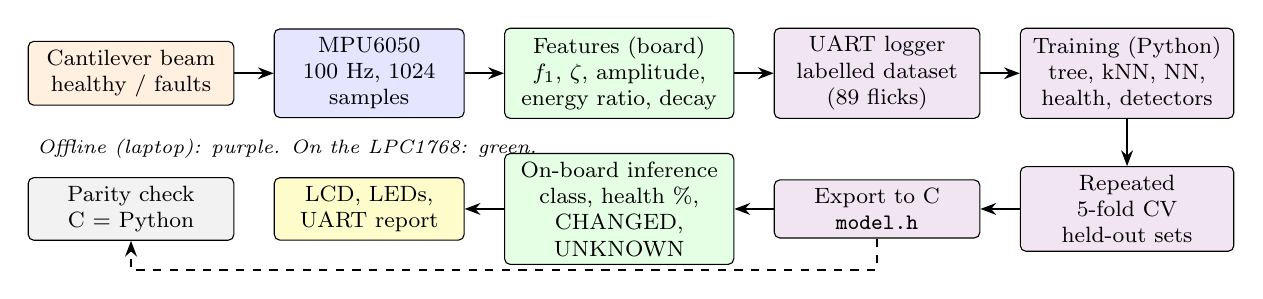
\begin{tikzpicture}[node distance=4mm and 5mm]
\node[blk, fill=orange!12, text width=24mm] (beam) {Cantilever beam\\healthy / faults};
\node[blk, fill=blue!10, right=of beam, text width=22mm] (acq) {MPU6050\\100 Hz, 1024 samples};
\node[blk, fill=green!10, right=of acq, text width=27mm] (feat) {Features (board)\\$f_1$, $\zeta$, amplitude,\\energy ratio, decay};
\node[blk, fill=violet!10, right=of feat, text width=24mm] (log) {UART logger\\labelled dataset\\(89 flicks)};
\node[blk, fill=violet!10, right=of log, text width=25mm] (train) {Training (Python)\\tree, kNN, NN,\\health, detectors};
\node[blk, fill=violet!10, below=6mm of train, text width=25mm] (val) {Repeated 5-fold CV\\held-out sets};
\node[blk, fill=violet!10, left=of val, text width=24mm] (exp) {Export to C\\\texttt{model.h}};
\node[blk, fill=green!10, left=of exp, text width=27mm] (inf) {On-board inference\\class, health \%,\\CHANGED, UNKNOWN};
\node[blk, fill=yellow!20, left=of inf, text width=22mm] (out) {LCD, LEDs,\\UART report};
\node[blk, fill=gray!10, left=of out, text width=24mm] (par) {Parity check\\C = Python};
\draw[arr] (beam) -- (acq);
\draw[arr] (acq) -- (feat);
\draw[arr] (feat) -- (log);
\draw[arr] (log) -- (train);
\draw[arr] (train) -- (val);
\draw[arr] (val) -- (exp);
\draw[arr] (exp) -- (inf);
\draw[arr] (inf) -- (out);
\draw[arr, dashed] (exp.south) -- ++(0,-4mm) -| (par.south);
\node[font=\scriptsize, below=0mm of beam.south west, anchor=north west, yshift=-3mm] {\textit{Offline (laptop): purple. On the LPC1768: green.}};
\end{tikzpicture}
\caption{Method approach: data collection, offline training and on-board deployment.}
\label{fig:approach}
\end{figure*}

\subsection{Test structure and fault cases}
The structure is a cantilever made of two 30 cm steel rulers (Fig.~\ref{fig:setup}). Ruler A projects 18.5 cm beyond the table edge and is held by a 10-inch screw G-clamp over a cardboard pad. Ruler B overlaps A by 13.5 cm and is joined to it by three binder clips, giving a free length of about 35.5 cm. The MPU6050 module is taped near the tip. Each measurement starts with a manual flick of the tip, after which the beam rings freely. The build needs no drilling or cutting, so the bench can be reassembled in any lab.

Three fault types were introduced (Fig.~\ref{fig:faults}). \emph{Added mass}: a Rs~20 and a Rs~5 coin taped together at the 28--30 cm mark. This is a change but not damage. \emph{Loose joint}: the middle binder clip removed (level 1), then one end clip removed as well (level 2). \emph{Loose support}: the G-clamp screw loosened in three steps of about 1/4, 1/2 and 3/4 turn; 3/4 turn is the loosest setting at which the beam still stays in place.

\begin{figure}[t]
\centering
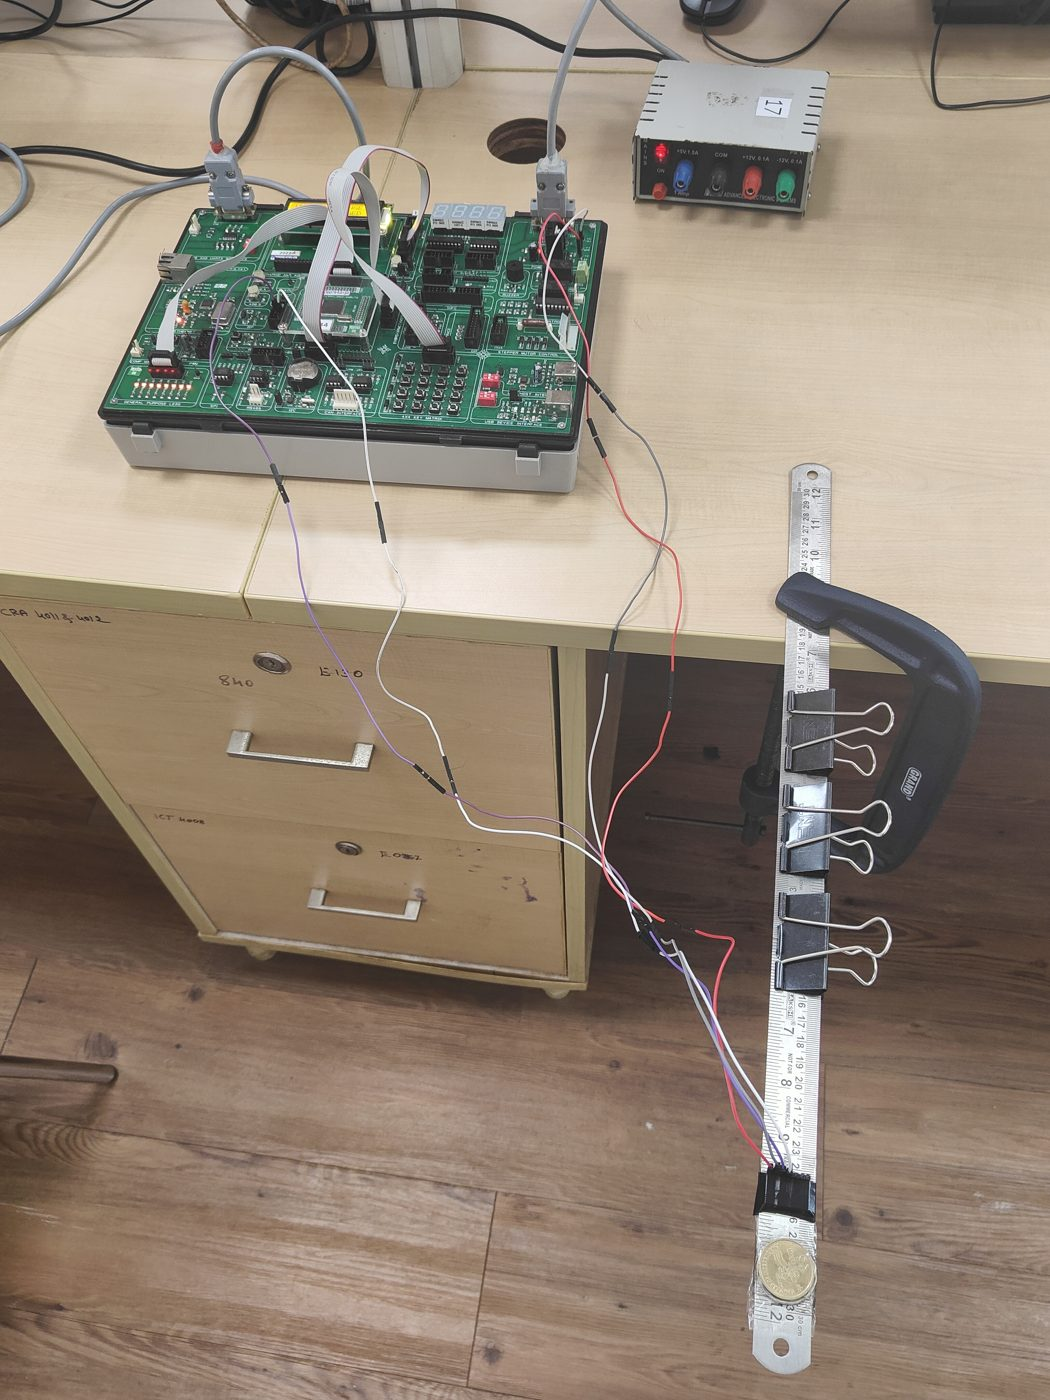
\includegraphics[height=40mm]{photo_setup_coin.jpg}\hfill
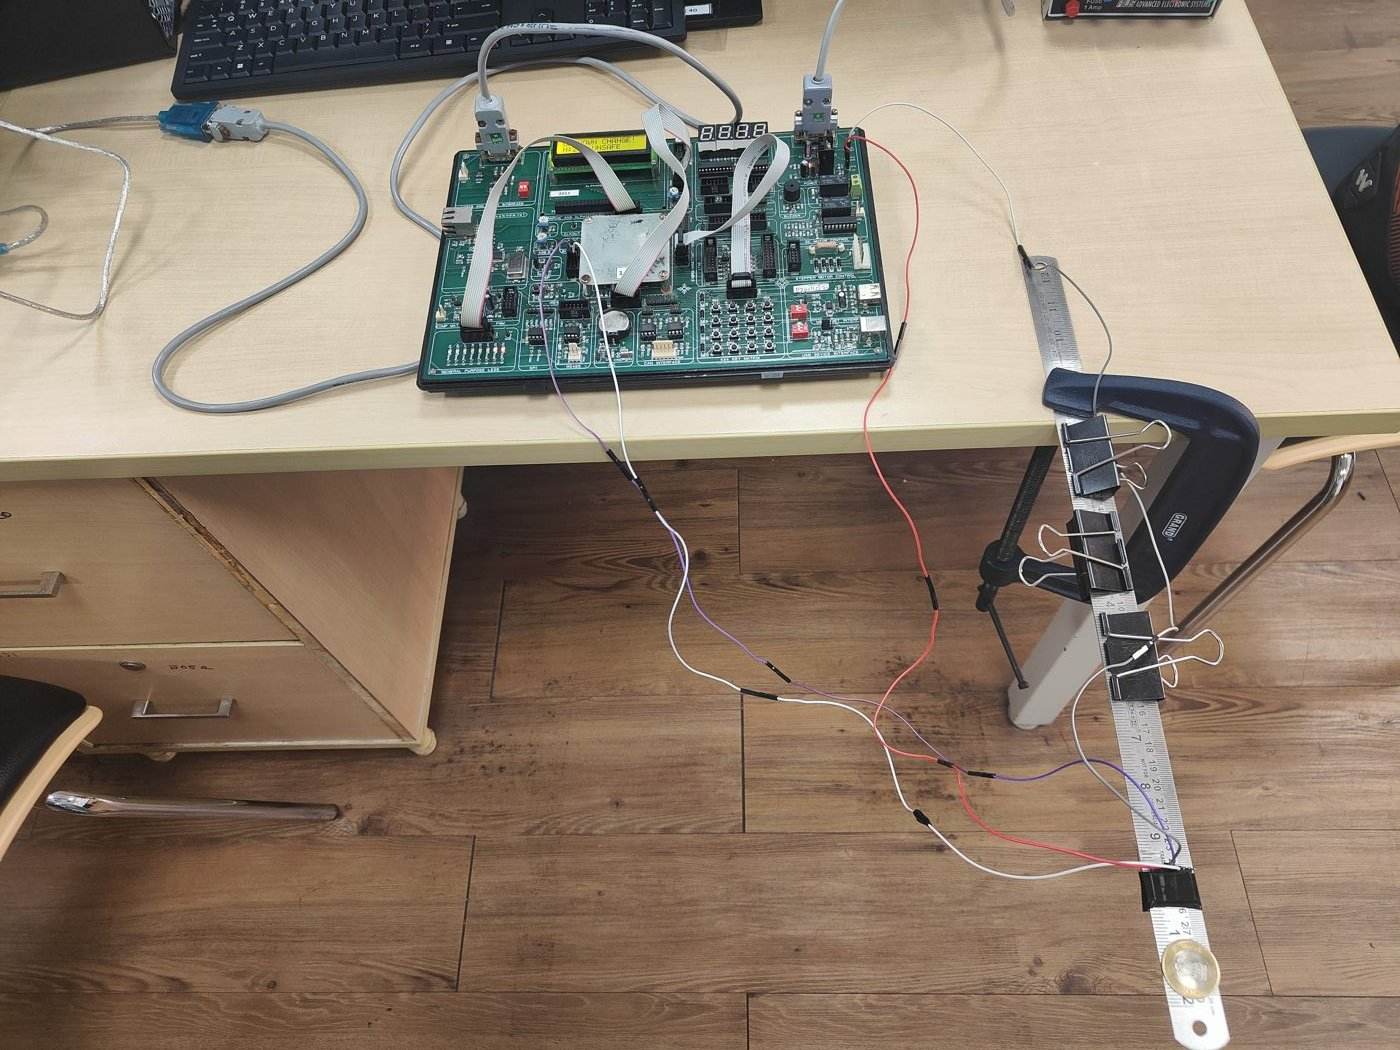
\includegraphics[height=40mm]{photo_setup_top.jpg}
\caption{Experimental setup. Left: LPC1768 board, power supply and the clamped two-ruler cantilever with the MPU6050 near the tip. Right: side view showing the three binder clips, the G-clamp and the wiring to the board.}
\label{fig:setup}
\end{figure}

\begin{figure}[t]
\centering
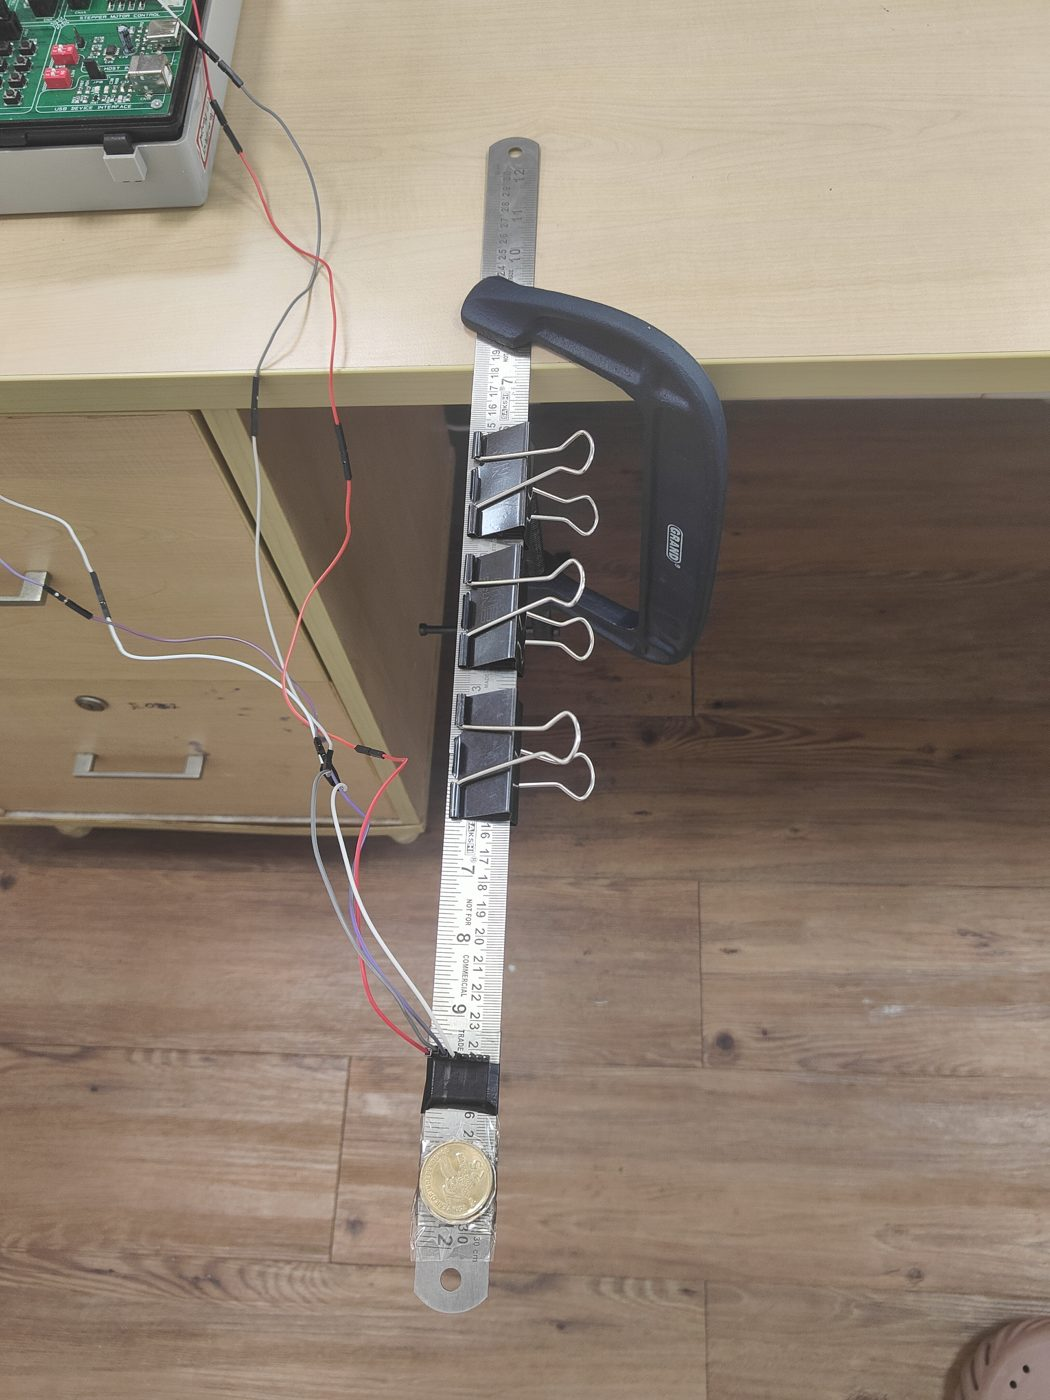
\includegraphics[height=48mm]{photo_coin_close.jpg}\hfill
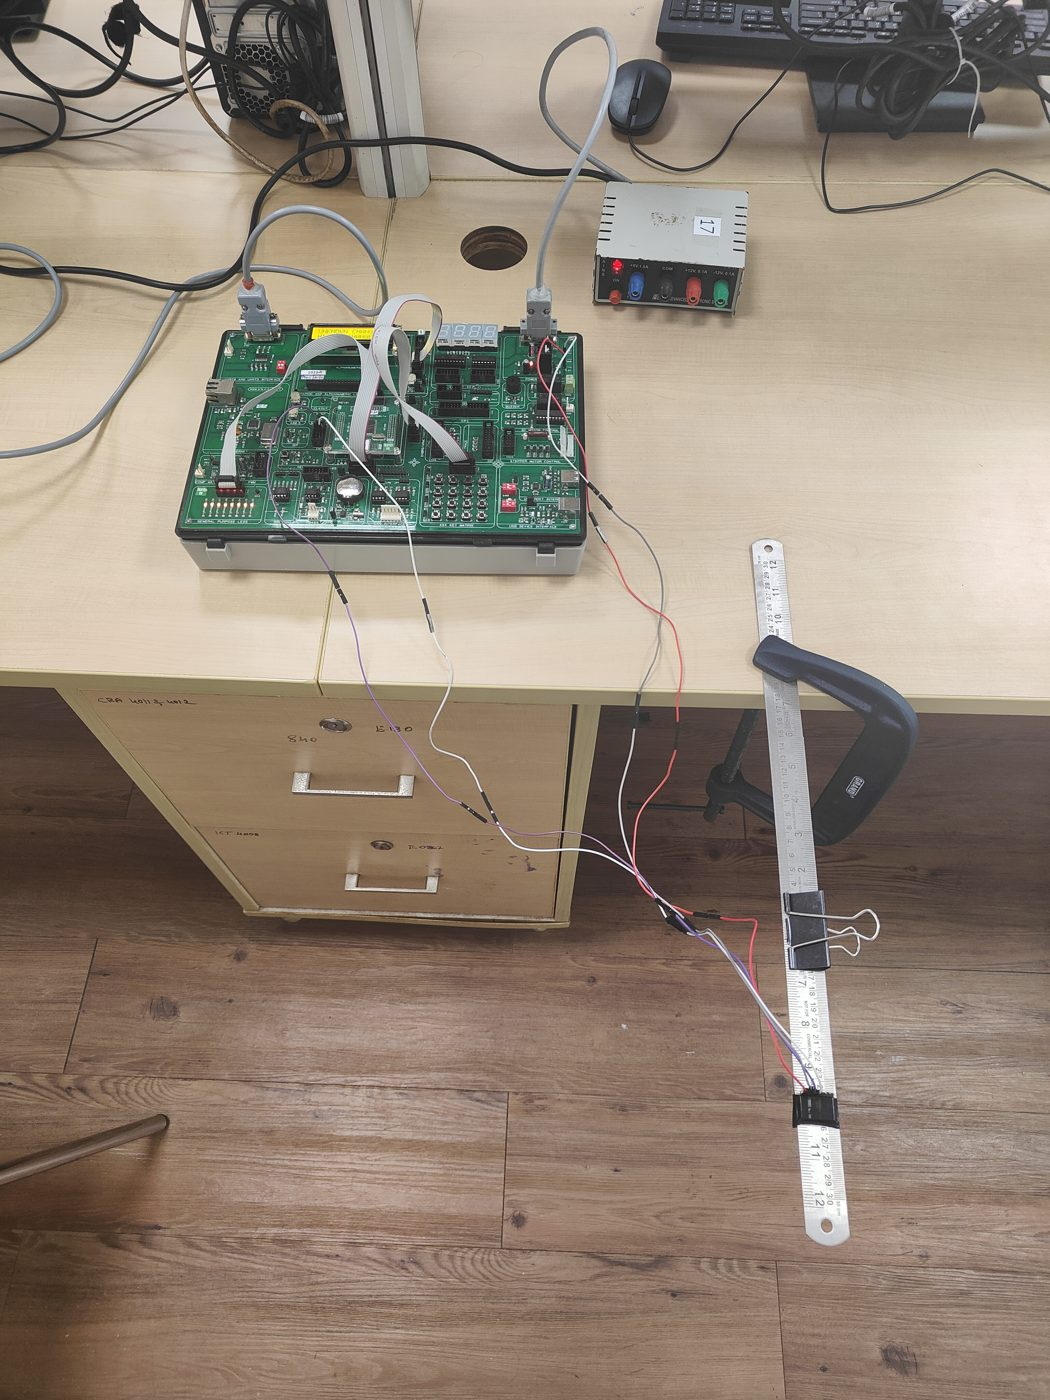
\includegraphics[height=48mm]{photo_joint_removed.jpg}
\caption{Fault cases. Left: added mass, coins taped beyond the sensor. Right: loose joint, clips removed from the ruler overlap.}
\label{fig:faults}
\end{figure}

\subsection{Hardware}
Fig.~\ref{fig:block} shows the block diagram. The LPC1768 (ARM Cortex-M3, 100 MHz, 512 KB flash, 64 KB SRAM) sits on the ALS-SDA-ARMCTXM3-01 development board. The MPU6050 is read over a software I\textsuperscript{2}C bus on two GPIO pins, with the range set to $\pm4$~g and the internal low-pass filter at 44 Hz to prevent aliasing. Timer~0 triggers a reading every 10 ms. The board's 16$\times$2 LCD shows the result, eight LEDs form a health bar, and the 4$\times$4 keypad selects calibration, teach mode and display pages. UART0 at 19200 baud sends every result and, while logging, the raw samples to the laptop.

\begin{figure}[t]
\centering
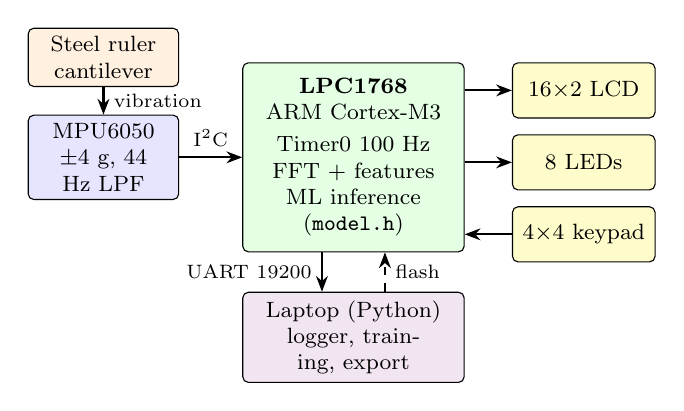
\begin{tikzpicture}[node distance=3.5mm and 4mm]
\node[blk, fill=orange!12, text width=17mm] (beam) {Steel ruler\\cantilever};
\node[blk, fill=blue!10, below=of beam, text width=17mm] (mpu) {MPU6050\\$\pm$4 g, 44 Hz LPF};
\node[blk, fill=green!10, right=8mm of mpu, text width=26mm, minimum height=24mm] (mcu) {\textbf{LPC1768}\\ARM Cortex-M3\\[2pt]Timer0 100 Hz\\FFT + features\\ML inference\\(\texttt{model.h})};
\node[blk, fill=yellow!20, right=6mm of mcu.north east, anchor=north west, text width=16mm] (lcd) {16$\times$2 LCD};
\node[blk, fill=yellow!20, below=2mm of lcd, text width=16mm] (led) {8 LEDs};
\node[blk, fill=yellow!20, below=2mm of led, text width=16mm] (key) {4$\times$4 keypad};
\node[blk, fill=violet!10, below=5mm of mcu, text width=26mm] (pc) {Laptop (Python)\\logger, training, export};
\draw[arr] (beam) -- node[right, font=\scriptsize]{vibration} (mpu);
\draw[arr] (mpu) -- node[above, font=\scriptsize]{I\textsuperscript{2}C} (mcu);
\draw[arr] (mcu.east |- lcd) -- (lcd);
\draw[arr] (mcu.east |- led) -- (led);
\draw[arr] (key) -- (mcu.east |- key);
\draw[arr] ([xshift=-4mm]mcu.south) -- node[left, font=\scriptsize]{UART 19200} ([xshift=-4mm]pc.north);
\draw[arr, dashed] ([xshift=4mm]pc.north) -- node[right, font=\scriptsize]{flash} ([xshift=4mm]mcu.south);
\end{tikzpicture}
\caption{Block diagram of the hardware.}
\label{fig:block}
\end{figure}

\begin{figure}[t]
\centering
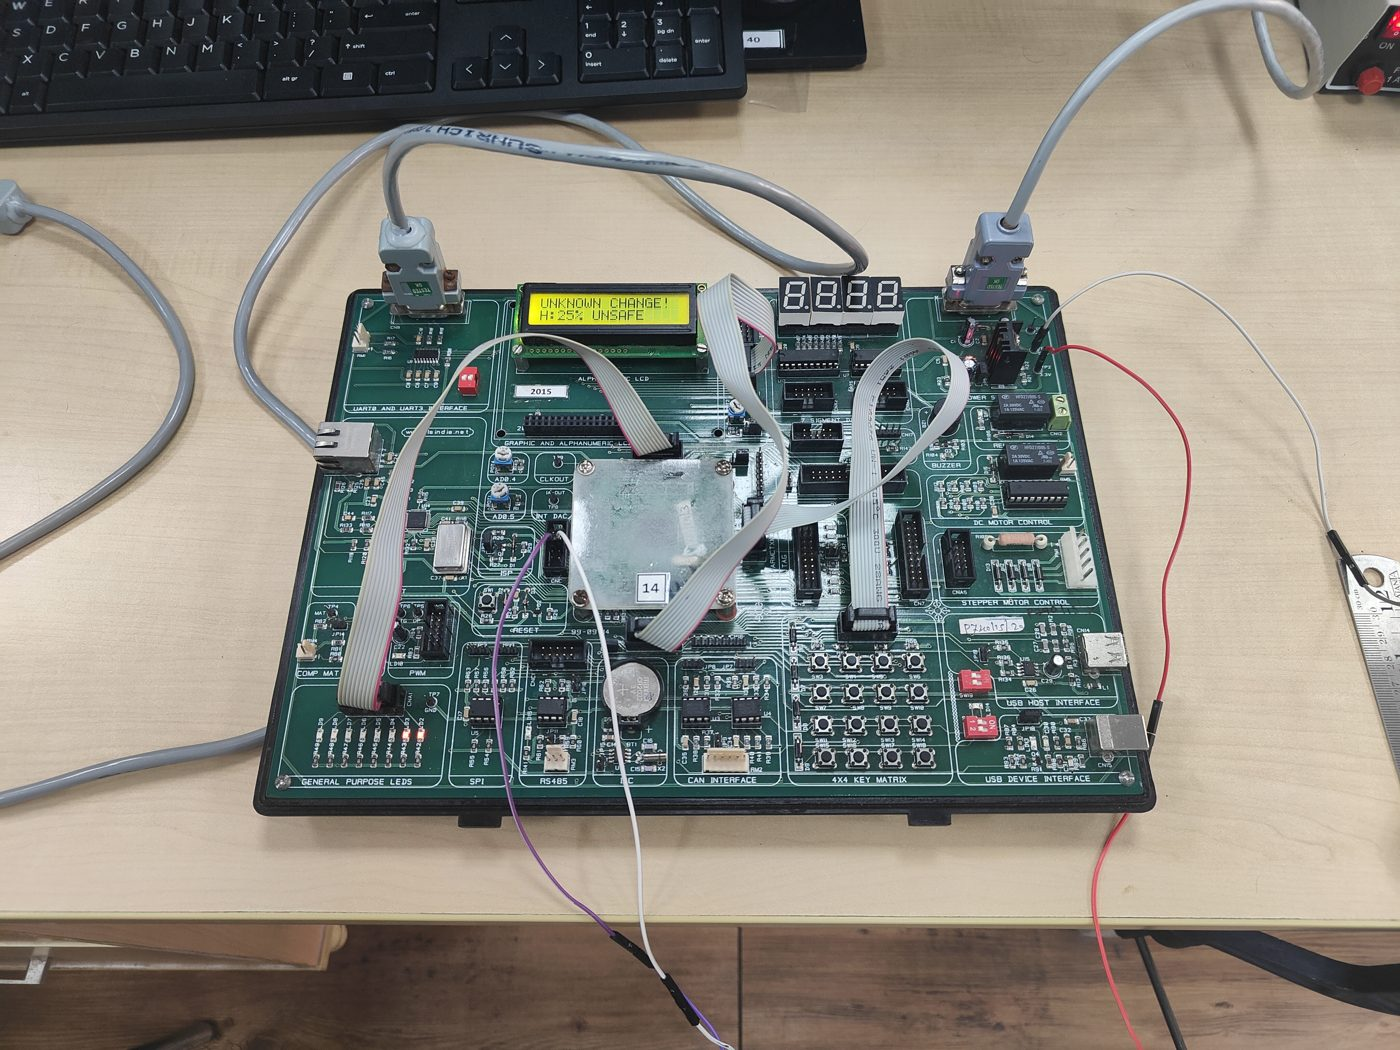
\includegraphics[width=0.95\linewidth]{photo_board_lcd.jpg}
\caption{LPC1768 board during a fault test. The LCD shows the change alarm and the health score.}
\label{fig:board}
\end{figure}

\subsection{Signal processing and features}
A flick is detected when the acceleration departs from its resting value by more than 0.3 g. The next $N=1024$ samples at $F_s=100$ Hz (10.24 s) are stored. The physical basis of the method is the single-degree-of-freedom model of the beam's first mode,
\begin{equation}
f = \frac{1}{2\pi}\sqrt{\frac{k}{m}},
\label{eq:sdof}
\end{equation}
so a loss of stiffness $k$ or a gain in mass $m$ lowers the natural frequency~\cite{hou2021}. After removing the mean, the record is multiplied by a Hann window to reduce spectral leakage,
\begin{equation}
w[n] = 0.5 - 0.5\cos\!\left(\frac{2\pi n}{N-1}\right),
\end{equation}
and transformed with a radix-2 FFT,
\begin{equation}
X[k] = \sum_{n=0}^{N-1} x[n]\,w[n]\,e^{-j2\pi kn/N},\qquad \Delta f = \frac{F_s}{N} = 0.098\ \text{Hz}.
\end{equation}
The largest bin $k_p$ between 3 and 40 Hz is refined with parabolic interpolation through its magnitude $\beta$ and its neighbours $\alpha$ and $\gamma$~\cite{belega2021}:
\begin{equation}
\delta = \frac{1}{2}\,\frac{\alpha-\gamma}{\alpha-2\beta+\gamma},\qquad f_1 = (k_p+\delta)\,\Delta f.
\label{eq:interp}
\end{equation}

Damping is taken from the free decay. For a lightly damped mode the amplitude decays as $A(t)=A_0e^{-\zeta\omega_1 t}$ with $\omega_1 = 2\pi f_1$. Taking logarithms gives a straight line, so the damping ratio is
\begin{equation}
\zeta = -\frac{s}{2\pi f_1},
\label{eq:damp}
\end{equation}
where $s$ is the least-squares slope of $\ln$ RMS against time, computed over 0.25 s windows from the loudest window until the RMS falls below 5\% of its peak. Three further features are the peak amplitude $a_{\max}$ (flick strength), the energy ratio
\begin{equation}
E_r = \frac{\sum_{k\in B} |X[k]|^2 - \sum_{|k-k_p|\le h} |X[k]|^2}{\sum_{k\in B} |X[k]|^2},
\end{equation}
which measures energy outside $\pm1$ Hz of the main peak (rattle and harmonics) within the band $B$ of 3--40 Hz, and the decay time $t_d$ until the RMS drops below 10\% of its peak. The feature vector is $\mathbf{x} = [f_1, \zeta, a_{\max}, E_r, t_d]$.

\subsection{Models}
All models use the standardised features $\tilde{x}_i = (x_i-\mu_i)/\sigma_i$.

\emph{Frequency-only baseline}: a depth-2 tree on $f_1$, representing the classical frequency-shift rule.

\emph{Decision tree}: CART of depth 3 with Gini impurity $G = 1-\sum_c p_c^2$; it is exported as nested \texttt{if} statements.

\emph{k-nearest neighbours}: $k=3$ with Euclidean distance over the 68 stored training flicks; new examples can be added on the board in teach mode.

\emph{Neural network}: a 5-8-4 multilayer perceptron,
\begin{equation}
\mathbf{h} = \max(0, W_1\tilde{\mathbf{x}}+\mathbf{b}_1),\quad \mathbf{p} = \operatorname{softmax}(W_2\mathbf{h}+\mathbf{b}_2),
\end{equation}
with 84 parameters; the largest $p_c$ is the predicted class and its value the confidence.

\emph{Health score}: each training condition has a damage level $d\in[0,1]$ (healthy 0, added mass 0, loose joint 0.5 and 1.0, loose support up to 0.75). The health of a new flick is
\begin{equation}
H = 100\left(1-\frac{1}{3}\sum_{j=1}^{3} d_j\right),
\end{equation}
where $d_j$ are the levels of its three nearest neighbours. $H<40$ is reported as UNSAFE.

\emph{Change detector}: the distance from the healthy baseline,
\begin{equation}
z = \sqrt{\frac{1}{5}\sum_{i=1}^{5}\left(\frac{x_i-\mu_i^{h}}{\sigma_i^{h}}\right)^2},
\end{equation}
flags CHANGED when $z>3$. The baseline $\mu^h,\sigma^h$ can be recalibrated on the board from ten healthy flicks (key C). \emph{Novelty detector}: UNKNOWN is shown when the nearest stored flick is farther than twice the 95th percentile of nearest-neighbour distances in the training set.

\emph{Trend}: the health of successive inspections is fitted with a line $H = a + b\,t$, and the step at which $H$ reaches 40 is predicted as $(40-a)/b$.

\subsection{Firmware flow}
Fig.~\ref{fig:flow} shows the firmware loop. All models are compiled from the exported header, so no training happens on the board.

\begin{figure}[t]
\centering
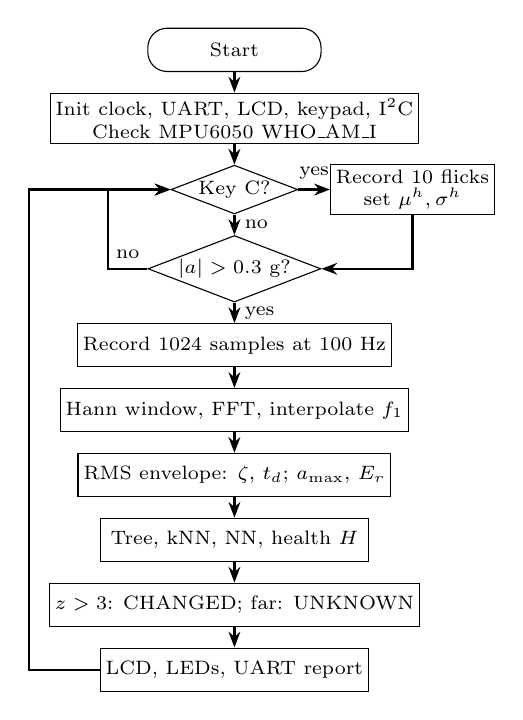
\begin{tikzpicture}[node distance=2.6mm]
\node[term] (start) {Start};
\node[proc, below=of start] (init) {Init clock, UART, LCD, keypad, I\textsuperscript{2}C\\Check MPU6050 WHO\_AM\_I};
\node[dec, below=of init] (cal) {Key C?};
\node[proc, right=4mm of cal, minimum width=20mm] (calib) {Record 10 flicks\\set $\mu^h,\sigma^h$};
\node[dec, below=of cal] (trig) {$|a|>0.3$ g?};
\node[proc, below=of trig] (rec) {Record 1024 samples at 100 Hz};
\node[proc, below=of rec] (fft) {Hann window, FFT, interpolate $f_1$};
\node[proc, below=of fft] (env) {RMS envelope: $\zeta$, $t_d$; $a_{\max}$, $E_r$};
\node[proc, below=of env] (ml) {Tree, kNN, NN, health $H$};
\node[proc, below=of ml] (det) {$z>3$: CHANGED; far: UNKNOWN};
\node[proc, below=of det] (outp) {LCD, LEDs, UART report};
\draw[arr] (start) -- (init);
\draw[arr] (init) -- (cal);
\draw[arr] (cal) -- node[above, font=\scriptsize]{yes} (calib);
\draw[arr] (cal) -- node[right, font=\scriptsize]{no} (trig);
\draw[arr] (calib) |- (trig);
\draw[arr] (trig) -- node[right, font=\scriptsize]{yes} (rec);
\draw[arr] (trig.west) -- node[above, font=\scriptsize]{no} ++(-5mm,0) |- (cal.west);
\draw[arr] (rec) -- (fft);
\draw[arr] (fft) -- (env);
\draw[arr] (env) -- (ml);
\draw[arr] (ml) -- (det);
\draw[arr] (det) -- (outp);
\draw[arr] (outp.west) -- ++(-9mm,0) |- (cal.west);
\end{tikzpicture}
\caption{Flowchart of the on-board firmware.}
\label{fig:flow}
\end{figure}

\subsection{Data collection and evaluation}
Each flick is labelled on the laptop and logged with its raw samples. Table~\ref{tab:data} lists the dataset. Before each fault the beam geometry was checked against a healthy reference; 24 flicks recorded with an incorrect ruler overlap of 15 cm were discarded. The first two support-loosening steps were kept out of training because their features lay inside the healthy spread (Section~IV-C); they are used only as a held-out test, together with five healthy re-check flicks. Accuracy is the mean of 5-fold stratified cross-validation repeated five times on the 68 training flicks.

\begin{table}[t]
\caption{Recorded dataset (medians)}
\label{tab:data}
\centering
\footnotesize
\setlength{\tabcolsep}{4pt}
\begin{tabular}{@{}lrrrl@{}}
\toprule
Condition & Flicks & $f_1$ (Hz) & $\zeta$ (\%) & Use \\
\midrule
Healthy & 30 & 4.74 & 2.92 & train \\
Added mass & 12 & 3.68 & 2.58 & train \\
Loose joint 1 & 10 & 4.47 & 2.67 & train \\
Loose joint 2 & 8 & 4.45 & 1.16 & train \\
Loose support 3/4 turn & 8 & 4.75 & 3.45 & train \\
Loose support 1/4 turn & 8 & 4.71 & 3.26 & held out \\
Loose support 1/2 turn & 8 & 4.75 & 3.13 & held out \\
Healthy re-check & 5 & 4.68 & 2.95 & held out \\
\midrule
Total & 89 & & & \\
\bottomrule
\end{tabular}
\end{table}

%=====================================================================
\section{Results and Discussion}
%=====================================================================
\subsection{Frequency estimation on the board}
Table~\ref{tab:freq} compares three frequency estimators against a 16$\times$ zero-padded FFT reference over all 89 flicks, with execution times measured on the LPC1768 using SysTick. Parabolic interpolation reduced the mean error from 0.027 Hz to 0.009 Hz, less than a tenth of the bin width, at no measurable extra time. Zero-crossing counting is 28 times faster but its mean error of 0.34 Hz is larger than the 0.27 Hz shift caused by a loose joint, so it cannot separate the classes (Fig.~\ref{fig:methods}). The FFT takes 117 ms, which is negligible against the 10.24 s recording.

\begin{table}[t]
\caption{Frequency estimators measured on the LPC1768}
\label{tab:freq}
\centering
\footnotesize
\setlength{\tabcolsep}{4pt}
\begin{tabular}{@{}lrrrr@{}}
\toprule
Method & Mean err. & Max err. & Time & RAM \\
\midrule
FFT peak bin & 0.027 Hz & 0.052 Hz & 116.9 ms & 8 KB \\
Interpolated FFT, \eqref{eq:interp} & \textbf{0.009 Hz} & 0.063 Hz & 116.9 ms & 8 KB \\
Zero-crossing & 0.338 Hz & 2.07 Hz & 4.2 ms & none \\
\bottomrule
\end{tabular}
\end{table}

\begin{figure}[t]
\centering
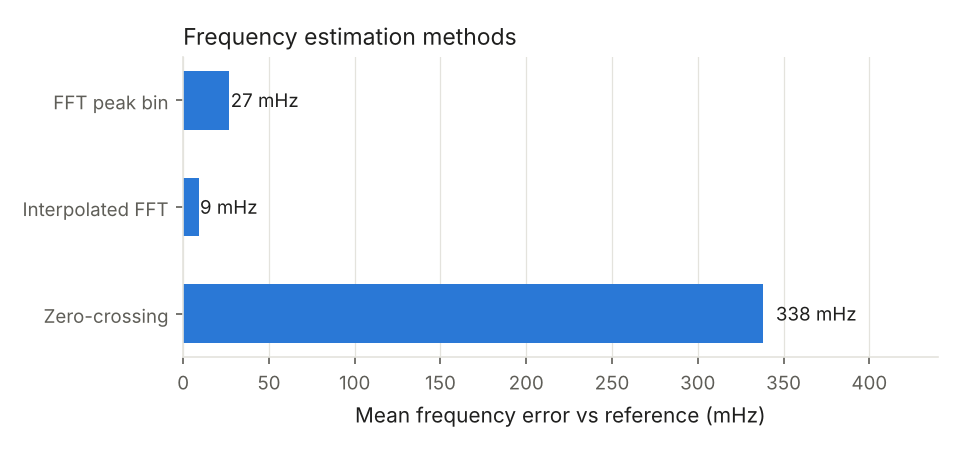
\includegraphics[width=\linewidth]{method_comparison.png}
\caption{Error and execution time of the three frequency estimators.}
\label{fig:methods}
\end{figure}

\begin{figure}[t]
\centering
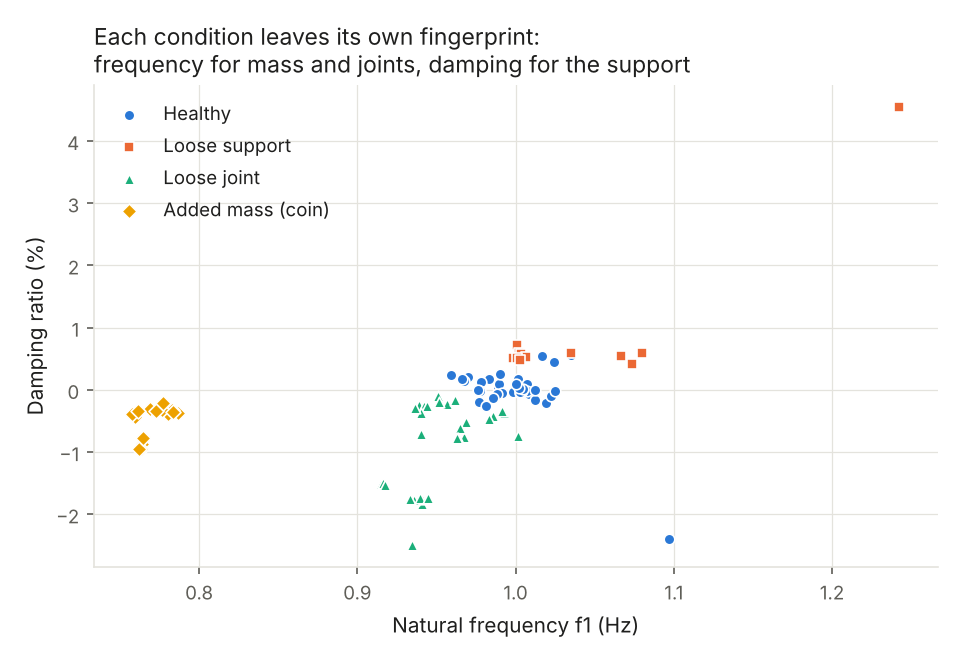
\includegraphics[width=\linewidth]{features_f1_vs_damping.png}
\caption{Damping against first natural frequency for all training flicks.}
\label{fig:fingerprint}
\end{figure}

\begin{figure}[t]
\centering
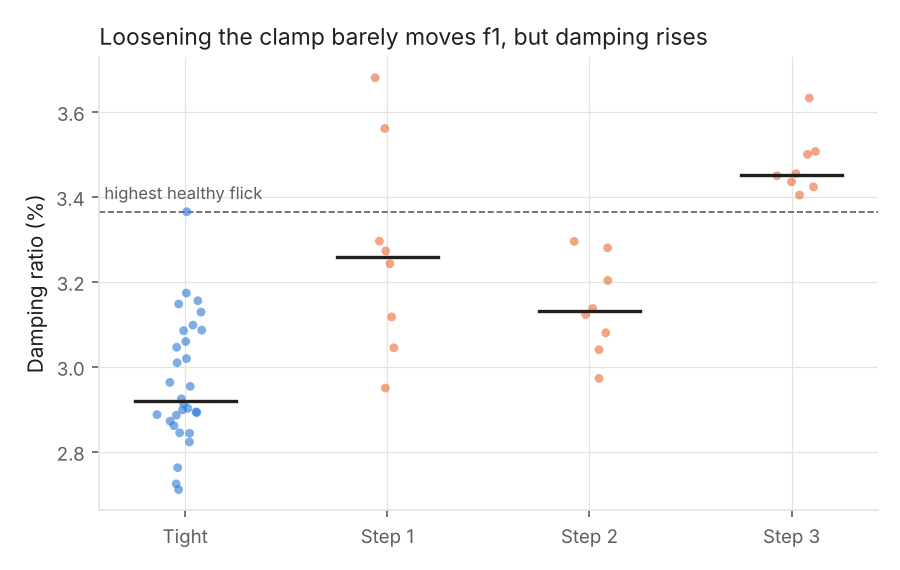
\includegraphics[width=\linewidth]{support_damping.png}
\caption{Damping ratio at each support-loosening step compared with the healthy range.}
\label{fig:support}
\end{figure}

\begin{figure}[t]
\centering
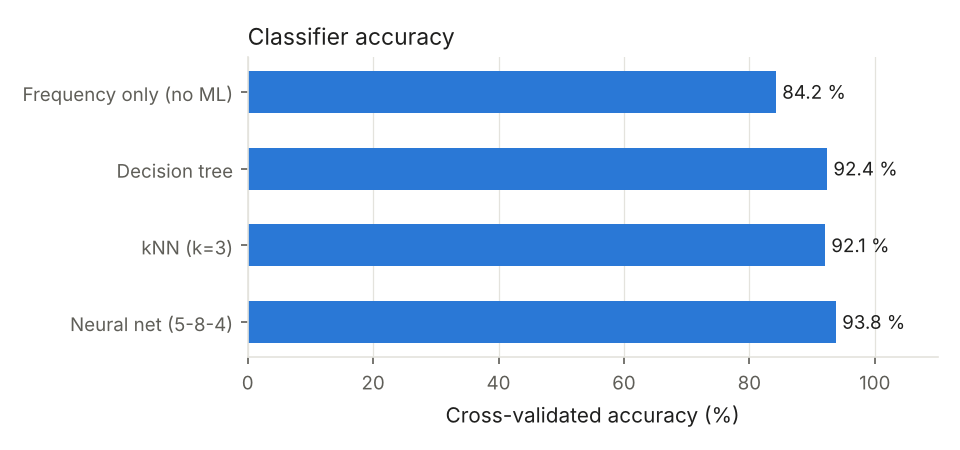
\includegraphics[width=\linewidth]{accuracy_comparison.png}
\caption{Accuracy of the frequency-only rule and the three classifiers.}
\label{fig:acc}
\end{figure}

\subsection{Each fault has its own signature}
Fig.~\ref{fig:fingerprint} plots damping against frequency for every flick. The added mass lowers $f_1$ by 22\%, as \eqref{eq:sdof} predicts for an increase in $m$. Removing clips lowers $f_1$ by about 6\% through a loss of joint stiffness, and removing the second clip also lowers damping from 2.9\% to 1.2\%, because less friction remains at the overlap. Loosening the support does not change $f_1$ at all (4.75 Hz against 4.74 Hz) but raises damping, since the loosely held end dissipates energy through friction, consistent with the loosening literature~\cite{huang2022}. A frequency-only method therefore cannot see this fault.

\subsection{Detection limit for support loosening}
Fig.~\ref{fig:support} shows damping at each loosening step. At 1/4 and 1/2 turn the damping lies inside the healthy spread, while at 3/4 turn every flick is above the highest healthy flick, with a median increase of 18\%. The screw clamp keeps gripping the ruler until it is almost released, so the first two steps are below the detection limit of this setup. On these held-out flicks the neural network labelled 4 of 8 and 3 of 8 as loose support, and the change detector fired once, which is consistent with features that sit on the boundary of the healthy cluster.

\subsection{Classification accuracy}
Table~\ref{tab:acc} and Fig.~\ref{fig:acc} give the cross-validated accuracy. All three ML models beat the frequency-only rule by 8 to 10 percentage points. The decision tree uses $f_1$ for 71\% of its splits and damping for 27\%, confirming that the gain comes from the damping feature. The confusion matrices in Fig.~\ref{fig:cm} show that most remaining errors are between healthy and loose support, the hardest pair. All five healthy re-check flicks were classified as healthy with no CHANGED alarm.

\begin{table}[t]
\caption{Cross-validated classification accuracy (4 classes)}
\label{tab:acc}
\centering
\footnotesize
\begin{tabular}{@{}lr@{}}
\toprule
Model & Accuracy \\
\midrule
Frequency only (depth-2 tree on $f_1$) & 84.2\% \\
Decision tree, depth 3 & 92.4\% \\
kNN, $k=3$ & 92.1\% \\
Neural network 5-8-4 & \textbf{93.8\%} \\
\bottomrule
\end{tabular}
\end{table}

\begin{figure}[t]
\centering
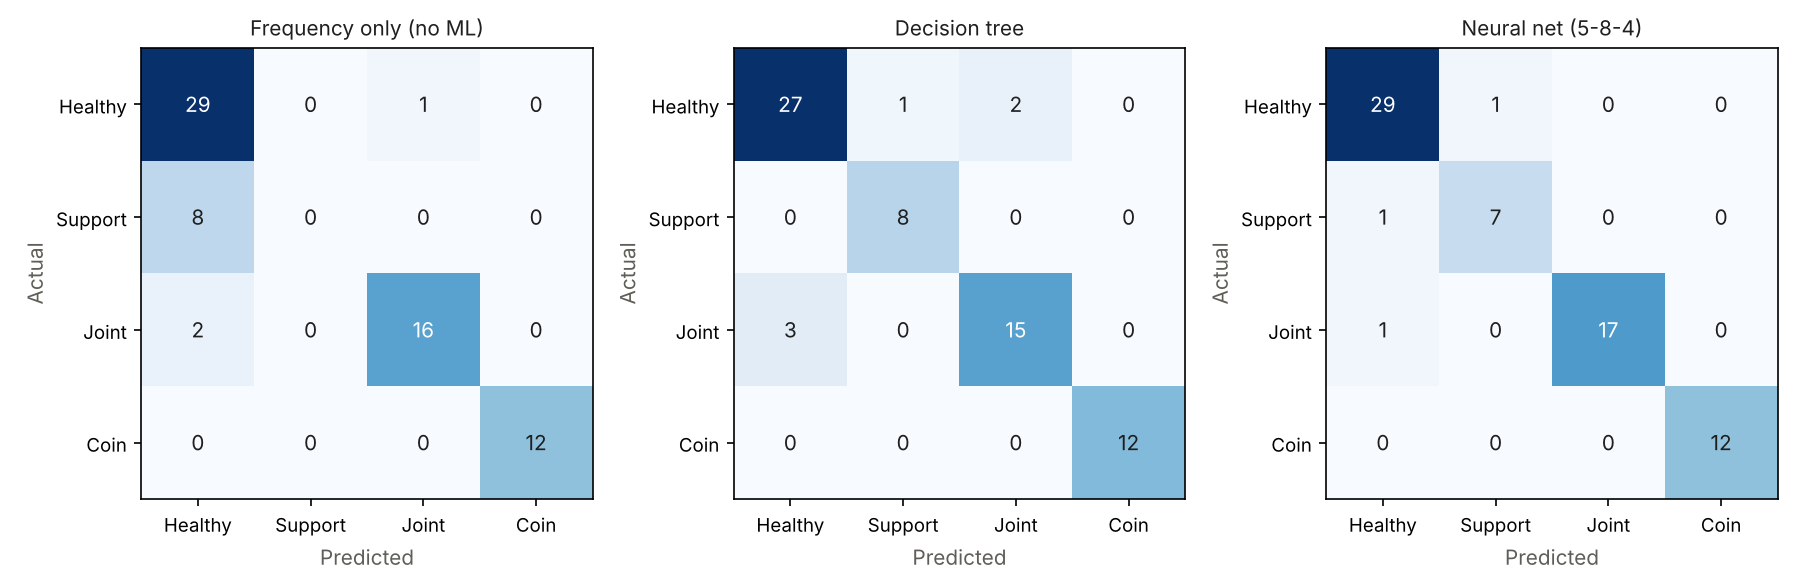
\includegraphics[width=\linewidth]{confusion_matrices.png}
\caption{Confusion matrices from cross-validation (left to right: frequency only, decision tree, neural network).}
\label{fig:cm}
\end{figure}

\subsection{Health score and trend}
The kNN health score had a mean absolute error of 5.6 points, against 17.8 points for linear regression on the same features (Fig.~\ref{fig:health}). In leave-one-out tests, healthy flicks scored 95.8 on average and none fell below the unsafe threshold. Over the support-loosening steps the mean health was 97, 66, 69 and 33. A line fitted to steps 0 to 2 predicted the beam would become unsafe at step 3.6; in the experiment it was unsafe at step 3, so the forecast was slightly late but in the right range (Fig.~\ref{fig:health}, right).

\begin{figure}[t]
\centering
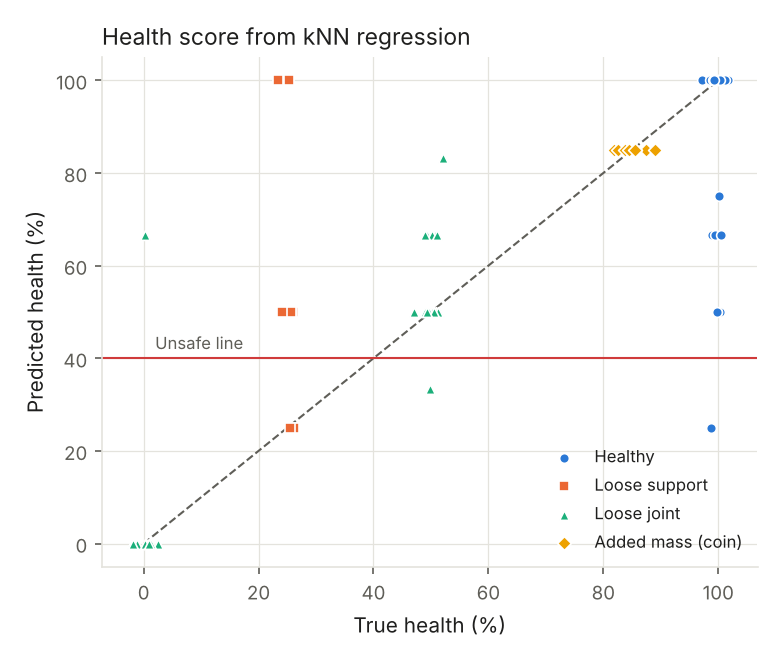
\includegraphics[width=0.49\linewidth]{health_score.png}\hfill
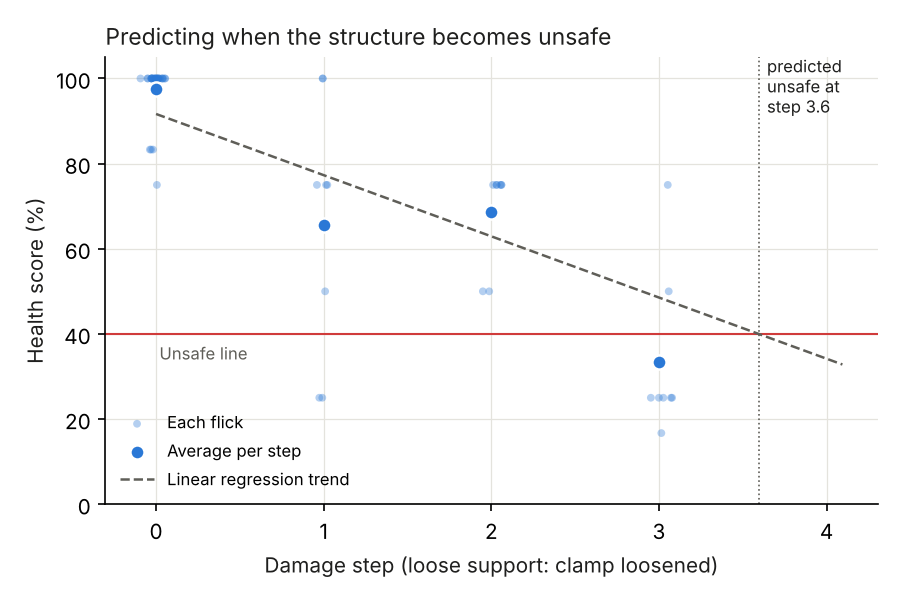
\includegraphics[width=0.49\linewidth]{trend.png}
\caption{Left: predicted against true health score. Right: health over successive loosening steps and the predicted unsafe point.}
\label{fig:health}
\end{figure}

\subsection{On-board operation}
The complete firmware, including the FFT, all six models and the training data needed by kNN, occupies about 20 KB of flash, within the 32 KB limit of the free Keil toolchain, and the FFT buffers use 8 KB of RAM. The C implementation was run on all 89 flicks on the PC and produced the same features and decisions as the Python reference for every flick. Fig.~\ref{fig:board} shows the board reporting a detected change and an unsafe health value during a fault test.

\subsection{Contributions verified through results}
Each claimed contribution is backed by a measured result. The assemble-only bench produced repeatable conditions: the healthy re-check after all faults gave 4.68 Hz against the original 4.74 Hz, and all five re-check flicks were classified healthy. The interpolated FFT on the Cortex-M3 measured frequency to within 0.009 Hz on average, ten times finer than the 0.098 Hz bin, in 117 ms. Adding damping and three other features raised four-class accuracy from 84.2\% for the classical frequency rule to 93.8\% with the neural network, and damping alone exposed support loosening, which left frequency unchanged and increased damping by 18\%. The kNN health score tracked damage severity with a mean error of 5.6 points and kept every healthy flick above the unsafe limit, and its trend forecast placed the unsafe point within one step of the observed one. Finally, the exported C models reproduced the Python features and decisions on all 89 flicks while using about 20 KB of flash. The experiment also set an honest limit: support loosening below about 3/4 turn could not be distinguished from the healthy state with this sensor and structure.

\subsection{Limitations}
The dataset is small (89 flicks) and comes from one structure in one room, so temperature and long-term drift were not studied. Flicks were applied by hand, which varies the amplitude; the amplitude feature absorbs this, but a mechanical exciter would give cleaner data. Only the first mode was used.

%=====================================================================
\section{Conclusion}
%=====================================================================
This paper showed that a complete vibration-based damage detection pipeline, from raw acceleration to a fault name, a health score and a trend forecast, can run on an entry-level ARM Cortex-M3 with a low-cost MEMS accelerometer. On a tool-free cantilever bench the system separated healthy, added-mass, loose-joint and loose-support conditions with 93.8\% accuracy, compared with 84.2\% for the classical frequency-shift rule, and the health score had a mean error of 5.6 points. The key finding is that damping, which the frequency rule ignores, is the only usable indicator of support loosening. All models fit in about 20 KB of flash and agree exactly with their PC reference. Future work will add a mechanical exciter, temperature compensation, higher modes from a second sensor and a larger multi-day dataset to lower the detection limit for early loosening.

\section*{Acknowledgment}
The authors thank their guides, Dr. G Pradeep Reddy and Pragya Jha, Assistant Professors, School of Computer Engineering, Manipal Institute of Technology, for their guidance, and the Embedded Systems Laboratory for the LPC1768 boards.

%=====================================================================
\IEEEtriggeratref{9}
\begin{thebibliography}{00}
\bibitem{gharehbaghi2022} V. R. Gharehbaghi, E. Noroozinejad Farsangi, M. Noori, T. Y. Yang, S. Li, A. Nguyen, C. M\'alaga-Chuquitaype, P. Gardoni and S. Mirjalili, ``A critical review on structural health monitoring: Definitions, methods, and perspectives,'' \emph{Archives of Computational Methods in Engineering}, vol. 29, no. 4, pp. 2209--2235, 2022, doi: 10.1007/s11831-021-09665-9.

\bibitem{hou2021} R. Hou and Y. Xia, ``Review on the new development of vibration-based damage identification for civil engineering structures: 2010--2019,'' \emph{Journal of Sound and Vibration}, vol. 491, Art. no. 115741, 2021, doi: 10.1016/j.jsv.2020.115741.

\bibitem{avci2021} O. Avci, O. Abdeljaber, S. Kiranyaz, M. Hussein, M. Gabbouj and D. J. Inman, ``A review of vibration-based damage detection in civil structures: From traditional methods to machine learning and deep learning applications,'' \emph{Mechanical Systems and Signal Processing}, vol. 147, Art. no. 107077, 2021, doi: 10.1016/j.ymssp.2020.107077.

\bibitem{flah2021} M. Flah, I. Nunez, W. Ben Chaabene and M. L. Nehdi, ``Machine learning algorithms in civil structural health monitoring: A systematic review,'' \emph{Archives of Computational Methods in Engineering}, vol. 28, no. 4, pp. 2621--2643, 2021, doi: 10.1007/s11831-020-09471-9.

\bibitem{bao2021} Y. Bao and H. Li, ``Machine learning paradigm for structural health monitoring,'' \emph{Structural Health Monitoring}, vol. 20, no. 4, pp. 1353--1372, 2021, doi: 10.1177/1475921720972416.

\bibitem{malekloo2022} A. Malekloo, E. Ozer, M. AlHamaydeh and M. Girolami, ``Machine learning and structural health monitoring overview with emerging technology and high-dimensional data source highlights,'' \emph{Structural Health Monitoring}, vol. 21, no. 4, pp. 1906--1955, 2022, doi: 10.1177/14759217211036880.

\bibitem{zonzini2020} F. Zonzini, C. Aguzzi, L. Gigli, L. Sciullo, N. Testoni, L. De Marchi, M. Di Felice, T. S. Cinotti, C. Mennuti and A. Marzani, ``Structural health monitoring and prognostic of industrial plants and civil structures: A sensor to cloud architecture,'' \emph{IEEE Instrumentation \& Measurement Magazine}, vol. 23, no. 9, pp. 21--27, 2020, doi: 10.1109/MIM.2020.9289069.

\bibitem{ray2022} P. P. Ray, ``A review on TinyML: State-of-the-art and prospects,'' \emph{Journal of King Saud University - Computer and Information Sciences}, vol. 34, no. 4, pp. 1595--1623, 2022, doi: 10.1016/j.jksuci.2021.11.019.

\bibitem{capogrosso2024} L. Capogrosso, F. Cunico, D. S. Cheng, F. Fummi and M. Cristani, ``A machine learning-oriented survey on tiny machine learning,'' \emph{IEEE Access}, vol. 12, pp. 23406--23426, 2024, doi: 10.1109/ACCESS.2024.3365349.

\bibitem{desousa2023} A. A. S. R. de Sousa, J. S. Coelho, M. R. Machado and M. Dutkiewicz, ``Multiclass supervised machine learning algorithms applied to damage and assessment using beam dynamic response,'' \emph{Journal of Vibration Engineering \& Technologies}, vol. 11, no. 6, pp. 2709--2731, 2023, doi: 10.1007/s42417-023-01072-7.

\bibitem{huang2022} J. Huang, J. Liu, H. Gong and X. Deng, ``A comprehensive review of loosening detection methods for threaded fasteners,'' \emph{Mechanical Systems and Signal Processing}, vol. 168, Art. no. 108652, 2022, doi: 10.1016/j.ymssp.2021.108652.

\bibitem{belega2021} D. Belega and D. Petri, ``Unbiased sine-wave frequency estimation by parabolic interpolation of DTFT samples,'' in \emph{Proc. IEEE Int. Instrumentation and Measurement Technology Conf. (I2MTC)}, 2021, pp. 1--5, doi: 10.1109/I2MTC50364.2021.9459910.

\bibitem{burrello2022} A. Burrello, G. Sintoni, D. Brunelli and L. Benini, ``Adversarially-trained tiny autoencoders for near-sensor continuous structural health monitoring,'' in \emph{Proc. IEEE 4th Int. Conf. Artificial Intelligence Circuits and Systems (AICAS)}, 2022, pp. 439--442, doi: 10.1109/AICAS54282.2022.9869952.

\bibitem{moallemi2023} A. Moallemi, R. Gaspari, F. Zonzini, L. De Marchi, D. Brunelli and L. Benini, ``Speeding up system identification algorithms on a parallel RISC-V MCU for fast near-sensor vibration diagnostic,'' \emph{IEEE Sensors Letters}, vol. 7, no. 9, pp. 1--4, 2023, doi: 10.1109/LSENS.2023.3303074.

\bibitem{capello2025} A. Capello, R. Berta, M. Fresta, L. Lazzaroni and F. Bellotti, ``Leveraging neural architecture search for structural health monitoring on resource-constrained devices,'' in \emph{Applications in Electronics Pervading Industry, Environment and Society}, Lecture Notes in Electrical Engineering. Cham, Switzerland: Springer, 2025, pp. 323--330, doi: 10.1007/978-3-031-84100-2\_38.
\end{thebibliography}

\end{document}
